%!TEX root = ../master.tex
\chapter{Introduction}
\label{chapter1_introduction}


Patterns, architectures, paradigms, frameworks, and languages change and evolve over time. The way we built software yesterday may not be suitable to serve the customers of tomorrow. In the 1990s, when the internet got traction, it was relatively easy to understand how servers and applications were connected. Usually, an application would run as a single server running on a single physical machine. If the network or power cable were disconnected, the application would become unreachable. \\

\noindent
As the popularity of the Internet grew, companies discovered a new opportunity and started to embrace the new market. These new markets included platforms such as Amazon (an online book retailer), eBay (an online auction service), and Hotmail (an online email service). The Internet boom in 1995 to 2000 led to more complex requirements for system development and architecture. The way software engineers usually dealt with these requirements were typically by adding functionality to an existing monolithic application. A monolithic architecture is an application where all functionality is packaged together as a single unit of compute or application. Chapter~\ref{chap:fundamentals_cloud_computing_architecture} covers the topic of monolithic applications in further detail. \\

\noindent
At the beginning of the 00s businesses faced new challenges by increasing demand for online services. The rapid growth and increased competition forced businesses into cutting costs and maximizing the utilization of existing technology \cite[p. 18]{endrei2004patterns}. Meanwhile, businesses still had to \textit{"continuously strive to serve customers better, be more competitive, and be more responsive to the business’s strategic priorities"} \cite[p. 18]{endrei2004patterns}. The two underlying factors behind these forces were the need to combine different technologies, \textit{heterogeneity}, and the need for \textit{change}. As a result, enterprises in the Internet business domain started adopting the idea of \textit{Service-Oriented Architectures (SOA)} instead of the old, homogeneous and monolithic architecture. Chapter~\ref{chap:fundamentals_cloud_computing_architecture} covers the topic of SOA in further detail. The paradigm shift in the architectural style is visualized in Figure~\ref{fig:paradigm_shift}.

\begin{figure}[H]
	\centering
	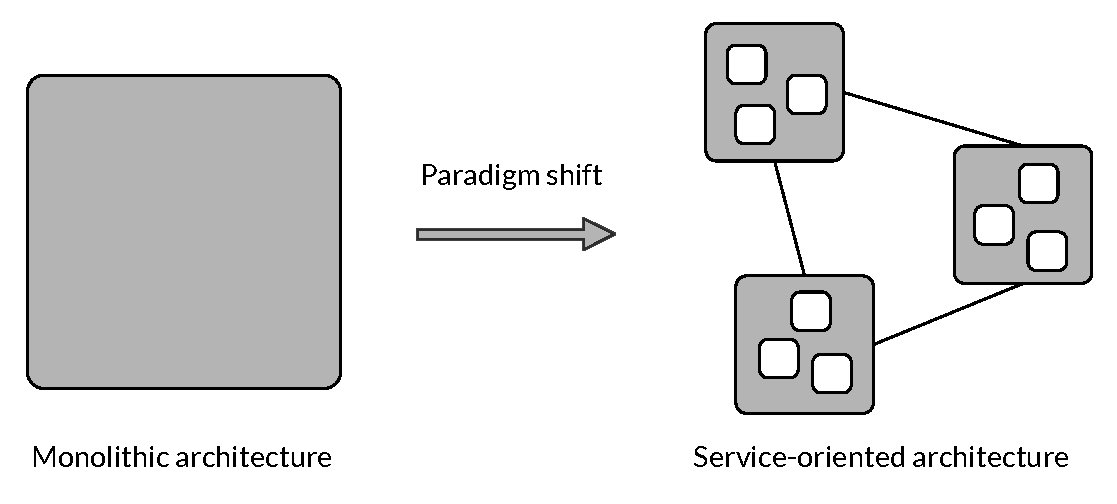
\includegraphics[width=8.5cm]{figures/paradigm_shift_monolithic_microservices}
	\caption{Paradigm Shift from Monolithic to Service-Oriented Architecture}
	\label{fig:paradigm_shift}
\end{figure}

\noindent
The need for heterogeneity arose because different types of systems had to be interconnected. Older systems and new services had to co-exist in this new architecture. Furthermore, this allowed businesses to develop new services across different platforms and languages. This new architectural style introduced the complexities of non-deterministic network calls. The paradigm shift from intra-process to inter-process communication added complexity to the developer's task, and the understanding of possible failures in distributed systems became crucial to ensure resilient systems. \\

\noindent
The other main force was the need for \textit{change}. Globalization and e-business were, at the beginning of the 00s, accelerating the pace of change. \textit{"Globalization leads to fierce competition, which leads to shortening product cycles, as companies look to gain advantage over their competition"} \cite[p. 18]{endrei2004patterns}. The increased competition forces businesses to be able to change quickly e.g. by adding new features. \\

\noindent
The offerings in the market control consumers' expectations. The fierce competition raises the expectations for online services. The increased expectations generate requirements to a service's solution. Developers are forced to improve techniques, tools, languages, etc. to satisfy these ever-increasing requirements, and in the end, meet the expectations of the consumers. How these forces impact a business is visualized in Figure~\ref{fig:customers_expectations}.

\begin{figure}[H]
	\centering
	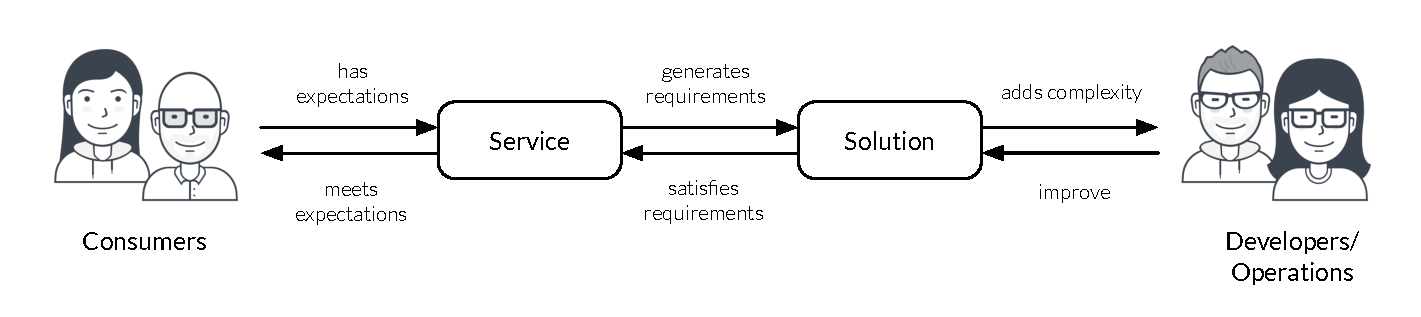
\includegraphics[width=\textwidth]{figures/paradigm_shift_why}
	\caption{Market Forces' Impact on Businesses}
	\label{fig:customers_expectations}
\end{figure}

\noindent
Consumers do not have much loyalty to Internet services \cite{iscoop-eu}. If a competitor offers a product of better quality or higher availability, the consumers will probably choose them instead. Furthermore, professor Klaus Schwab describes this need for change:

\begin{citat} []
"In the new world, it is not the big fish which eats the small fish, it’s the fast fish which eats the slow fish." \textbf{- Professor Klaus Schwab, Founder and Executive Chairman of the World Economic Forum} \cite{schwab2015techrevolusion}
\end{citat}


\noindent Through the 00's the service-oriented architecture trend continued to grow, and much new technology was developed and implemented. Popular protocols such as \textit{Simple Object Access Protocol (SOAP)} and the infamous \textit{Enterprise Service Bus (ESB)} were adopted. Chapter~\ref{chap:fundamentals_cloud_computing_architecture} discusses these protocols in further details. In 2011, a group of software architects started to discuss what they saw as a common architectural style they recently had been exploring. In 2012, James Lewis, Principal Consultant at ThoughtWorks, presented the ideas as \textit{microservices} the UNIX way. Around the same time Fred George, Independent Consultant and former Vice President at ThoughtWorks, presented the same idea, and Adrian Cockcroft, Cloud Architect at Netflix, presented the ideas that Netflix had been working with as \textit{'fine-grained services'}. \\

\noindent
The reason for these new enterprise architectural styles was the direction that the SOA community had taken. Too much logic centralized in middleware components, too little focus on a decomposition of the business domain, and focus on reusability rather than isolation and autonomy. \\

\noindent
The introduction of cloud computing (widely accessible) in 2006 by Amazon Web Services Elastic Compute Cloud  (AWS EC2) as a commercial web service allowed companies to rent computer resources online to host their infrastructures and applications \cite{history_of_cloud_computing}. The key enabling factors behind this were the improvement of virtualization technologies and proper abstractions of the underlying hardware. The evolution of cloud computing along with the service-oriented paradigm shift allowed a more fine-grained architectural trend. The fine-grained trend was further fostered by the spread of container technology in 2013 when Docker was released. Internally Google has used container technology together with a cluster management system, Borg, since 2004 \cite[p. 1]{verma2015borg}. Kubernetes, an open source cluster management system built on the experiences of running and managing containers for a decade, was released by Google in 2014. The next evolutionary step, according to Google, is to transform data centers from being machine-oriented to being application-oriented by using containers \cite[p. 5]{burns2016borg_omega_kubernetes}. Bill Baker, Distinguished Engineer at Microsoft, described the transformation with an analogy of treating servers as cattle instead of pets. \\


\noindent
The demand for engineers with skills in cloud computing and this new way of building distributed applications is increasing \cite{newyorktimesclouddemand}. This new paradigm demands different skills and an understanding of distributed systems. The demand for graduates with knowledge and expertise in these topics is increasing. Unfortunately, many educational institutions have not offered courses within this new paradigm. As Breivold and Crnkovic point out:

\begin{citat} []
"The existing Cloud Computing courses reported in literatures do not address enough details and cloud-related topics that are required in terms of building cloud-based architectures, developing and migrating applications in a cloud. They also lack utilization of real-world systems." \textbf{- Breivold and Crnkovic, 2014} \cite[p. 36]{breivold2014education_strategies}
\end{citat}


\noindent
The lack of education is partly because of the rapid pace of change in cloud computing and the the fact that the industry mainly drives the research. The absence might lead to students graduating without the skill set required by the industry.  \\

\noindent
Abstraction makes it easier for developers and operation personnel to manage cloud solutions. Abstractions are good - however failing to understand the premise of the abstractions and the underlying environment may result in catastrophic consequences.  \\

\noindent
Before cloud computing, it was relatively easy to understand how an application would run on a single physical machine. If the machine was unreachable, the service would be unreachable. Today's massive distributed systems are now powering the cloud. Monolithic applications are still widespread. However, microservices and containers are on the verge of hitting mainstream adoption according to a survey done by Nginx with 1800 IT professionals \cite{nginx2016future}. Therefore, there is a need to align the mismatch between the mental model of the graduates and the demand in the industry. This mismatch is visualized in Figure~\ref{fig:mental_model_present}.

\begin{figure}[H]
	\centering
	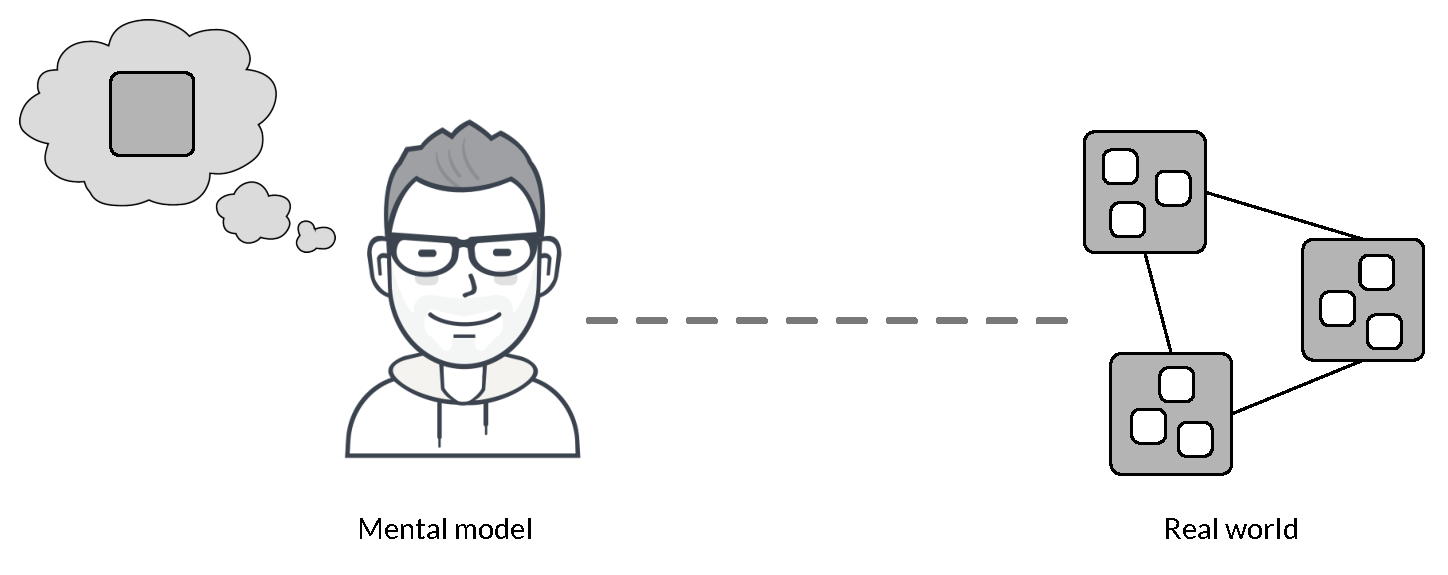
\includegraphics[width=10cm]{figures/present_mental_model}
	\caption{Mental Model Mismatch}
	\label{fig:mental_model_present}
\end{figure}

\noindent
Even though the interest in academia is growing, the demand for students with an understanding of this paradigm is currently not met. Furthermore, Breivold and Crnkovic express the need for graduates who understand the non-deterministic behavior, faults in a distributed system, and the need for designing highly-available and resilient systems. Nygard describes these undesired effects in distributed systems as antipatterns and presents patterns to avoid these undesired effects \cite[p. 31-114]{nygard2007release}. \\

\noindent
Designing for resilience in microservice architecture is therefore of utmost importance to meet consumers' expectations and thereby to the business.


\section{Motivation}

The cloud computing paradigm changes the way consumers and businesses interact. Marc Andreessen, co-founder of Venture capital firm Andreessen-Horowitz\footnote{investor in Facebook, Skype, Twitter, among others}, stated in 2011 that \textit{"software is eating the world"} \cite{andreessen2011eating}. Meaning that every company is becoming a software company to some degree. Even though the interest of cloud computing in academia is on the rise, it does not meet the demand of the industry. Cloud computing will have a bigger role in the industry in the coming years, and therefore, it becomes a part of the mandatory skill set for professionals \cite[p. 30]{breivold2014education_strategies}.
Education in this field needs to follow the technological advances and required skill set from the industry. There is thus a need for alignment of the mental model of graduates and the real world. \\

\noindent
The motivation for this master's thesis is, therefore, to investigate how these two can be aligned. Furthermore, this master's thesis will investigate how educators can be able to demonstrate and highlight the non-deterministic behavior of distributed systems.


\section{State of the Art}
\label{sec:sota}

\subsection*{Cloud Computing Education Strategies \cite{breivold2014education_strategies}}
Breivold and Crnkovic propose education strategies for cloud computing to meet the demand from the industry. They emphasize a strong need in course design to fulfill the following requirements: \textit{"(i) clarify cloud computing concepts, (ii) include underlying technologies targeting different roles in a cloud,  (iii) integrate both educator's goals and practitioner's objectives"}. \\

\noindent
Furthermore, they stress the importance of academia/industry partnerships and the multiplicity of learning styles such as readings, class discussions, guest lectures, and hands-on projects.

\subsection*{TeachCloud: A Cloud Computing Educational Toolkit \cite{jararweh2013teachcloud}}

Jararweh et al identified the lack of teaching tools in cloud computing education. They conducted a survey, after completing a cloud computing course, to identify the challenges students found most important. 93\% of the students answered that the lack of hands-on experience was the largest challenge.\\

\noindent
Jararweh et al propose a modeling and simulation environment to accommodate this lack of teaching tools. A toolkit called TeachCloud was developed. TeachCloud is an extension of CloudSim that enables experimenting with different components such as processing elements, data centers, virtualization, and web-based applications.
TeachCloud made it easy for students to modify cloud computing components and gave them deeper insights into the factors that affect cloud computing environments.


\subsection*{The Glasgow Raspberry Pi Cloud: A Scale Model for Cloud Computing Infrastructures \cite{tso2013glasgow}}
Tso et al describe that most research into cloud computing \textit{"relies on either limited software simulation, or the use of a testbed environment with a handful of machines"}.
They present a scale-model of a data center consisting of Raspberry Pis (PiCloud). The Raspberry Pi has made the construction of a scale-model affordable because of its low cost and its low power consumption.
PiCloud emulates all layers of a cloud stack, and provides a full-featured cloud computing research and education environment.
PiCloud is divided into four racks each containing 14 Raspberry Pi model B which sums to a total of 56 nodes.
Tso et al conclude that the PiCloud enables them to carry out practical research without the limitations of simulation.


\subsection*{Affordable and Energy-Efficient Cloud Computing Clusters: The Bolzano Raspberry Pi Cloud Cluster Experiment \cite{abrahamsson2013bolzano}}
Abrahamsson et al state that \textit{"today's students who are the researchers of tomorrow, are not getting enough exposure to real cloud computing infrastructures"}. They emphasize that students need hands-on experience in this area. However, acquiring such an infrastructure is too expensive for universities, and they propose building a Raspberry Pi consisting of 300 nodes instead. \\
Furthermore, Abrahamsson et al highlight the two most important use-cases for the cluster: being an inexpensive and green testbed for cloud computing research, and a robust and mobile data center for operating in adverse environments.


\subsection*{Iridis-pi: a low-cost, compact demonstration cluster \cite{cox2014iridis}}
Iridis-Pi cluster consists of 64 Raspberry Pi model B. Cox et al emphasize the benefits as low power consumption, easy portability, affordability, and ambient cooling. Iridis-Pi is suitable for educational use and provides students with a platform for inspiration and experimentation with high-performance computing.
Cox et al have built Iridis-Pi and performed benchmarks on the computation performance with e.g. Hadoop.


\section{Problem Formulation}

\textit{The demand for software engineers who understand cloud computing and the complexities of distributed systems is strongly increasing, meanwhile many universities do not offer education within these areas. Teaching in this fairly new discipline is, therefore, important in order to prepare students for the challenges in the job market, but realistic experimenting with the technologies behind the cloud providers is expensive. Is it possible to build a small-scale model of a cloud computing environment using modern technologies? Does it make sense to build a small-scale cloud computing environment for teaching? How can a small-scale tangible cloud computing environment support students’ learning? How can a small-scale tangible cloud computing cluster clarify the complexities and possible faults in a distributed system? Moreover, can such a cluster be used for research and experiments? } \\

\noindent\textit{The answer to these questions will impact how cloud computing courses are designed and taught, and thereby disclose the value of a small-scale tangible cloud computing cluster as an inexpensive learning object.} \\

\noindent\textit{Courses have been designed using simulations or leveraging cloud providers, but, to our knowledge, there have not been other attempts to incorporate hands-on experience in cloud computing courses. The effects of hands-on teaching methods are, thereby, missing.} \\

\noindent\textit{This present master’s thesis will examine how a small-scale tangible cloud computing cluster can support students’ learning. In order to do so a course will be designed and conducted, furthermore a tangible cluster will be designed and built. The clusters will be handed out in order to enable the students to get a hands-on experience with cloud computing and conduct experiments with different software architectures. Several experiments will be designed and conducted in order to determine the students’ learning outcome, clarify the importance of designing for failure, and the cluster’s role therein.}

\section{Our Contribution}


We argue that the evolution of cloud computing needs more focus in the academic community. There is a need for finding a better way to learn and grasp the complexities of cloud computing and microservice architectures. TeachCloud proposed the idea of using simulations as an educational tool, and other unconventional methods such as using a Raspberry Pi cluster has been taken. We propose a small-scale tangible cloud computing cluster, KubeCloud, as a small scale model of a cloud computing infrastructure to be part of the education of engineering and computer science students. KubeCloud helps to emphasize the problems and fallacies of distributed computing in a cloud computing environment. \\

\noindent Building on the pedagogy and theories of how to optimize student learning, specifically within engineering education, we see a need for a hands-on tangible computing cluster to educate and foster further research within the area of cloud computing. KubeCloud acts as a mediator object to align the students' mental model with the real world as depicted  in Figure~\ref{fig:mental_model_future}

\begin{figure}[H]
	\centering
	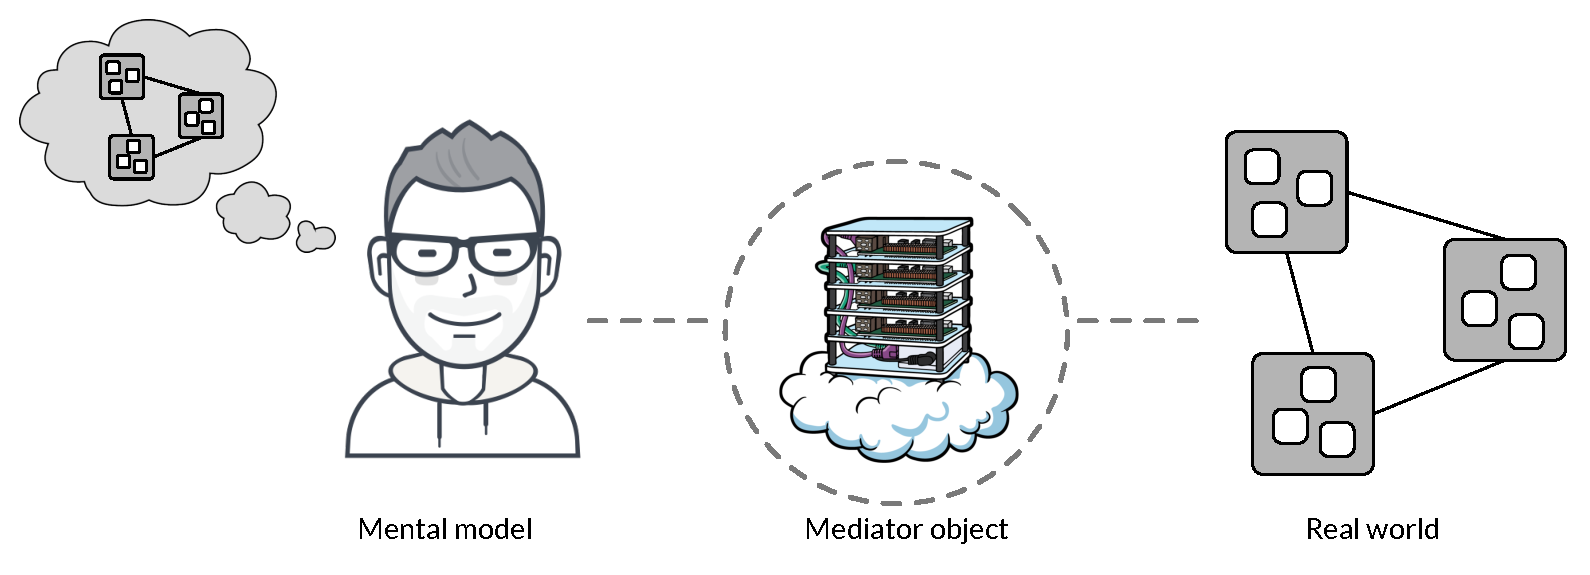
\includegraphics[width=10cm]{figures/mental_model_future}
	\caption{Mental Model after Designed Learning Activity}
	\label{fig:mental_model_future}
\end{figure}

\noindent
The mediating role of KubeCloud will help students understand the underlying assumptions and concepts of cloud computing. KubeCloud will furthermore provide a basis for experimentation and research in a controlled test environment. Allowing for verification of e.g. Nygard's stability patterns to highlight the importance of building resilient systems and designing for failure.

\section{Reading Guide and Structure}
This master's thesis consists of ten chapters, as visualized in Figure~\ref{fig:thesis_structure}. The solid lines indicate the suggested order of reading. Furthermore, seven appendices are created to assist the reader and provide more detailed descriptions of specific topics. The dashed lines in Figure~\ref{fig:thesis_structure} indicates the order in which the Appendices should be read. \\

\noindent\textbf{Chapter 2 - Fundamentals of Learning Theory}: Learning theory is an important part of aligning students' mental model with the real world. Knowing how engineering students learn becomes a vital part of designing a learning activity and a learning object. \\

\noindent\textbf{Chapter 3 - Designing the Learning Activity}: Designing a learning activity is necessary to investigate the effects of KubeCloud. Learning theories must be applied within the constraints of the course format.\\

\noindent\textbf{Chapter 4 - Fundamentals of Cloud Computing Infrastructure}: An understanding of cloud computing infrastructure fundamentals is necessary to design and build a learning activity and a tangible cloud computing cluster. \\

\noindent\textbf{Chapter 5 - Fundamentals of Cloud Computing Architecture}: Cloud computing has enabled new ways of designing architectures. An understanding of cloud architecture fundamentals is, therefore, necessary to design and build a learning activity and a tangible cloud computing cluster. \\

\noindent\textbf{Chapter 6 - Defining Resilient Cloud Computing}: Microservices have introduced the non-determinism of distributed network communication. It is therefore of utmost importance to understand the complexities of distributed systems to build resilient systems. \\

\noindent\textbf{Chapter 7 - Building a Tangible Cloud Computing Cluster}: Visualization and tangibility are important in conveying cloud computing concepts to accomodate engineering students' learning style preferences. Designing and implementing a tangible cloud computing cluster as a mediating learning object to align the students' mental model to the real world is needed.\\

\noindent\textbf{Chapter 8 - Experiment: Evaluating Application Level and Infrastructure Level Resilience}: KubeCloud allows for physical experimentation that cannot be done using cloud providers. Experimenting with resilience at the infrastructure and application level is a key feature in order to demonstrate the new paradigm of embracing failure. \\

\noindent\textbf{Chapter 9 - Experiment: Evaluation of KubeCloud and Course Design}: An evaluation is needed to determine whether KubeCloud and the designed course is a viable cloud computing teaching strategy for engineering students. \\

\noindent\textbf{Chapter 10 - Conclusions}: A presentation of the lessons learned is needed in order to draw the overall conclusion of the effects of the designed learning activity and KubeCloud as a learning and research object. \\

\noindent\textbf{Appendix A - Designing the Learning Activity}: Presents an overview of materials created and selected for designing the learning activity.  \\

\noindent\textbf{Appendix B - Additional Kubernetes Concepts}: Presents further concepts of Kubernetes, such as canary deployments, scaling, YAML examples, and database opportunities. \\

\noindent\textbf{Appendix C - Characteristics and Principles of Microservice Architecture}: Describes the characteristics and principles of Microservices in greater detail. \\

\noindent\textbf{Appendix D - Physical Design of KubeCloud}: Presents additional images and drawings of the physical design of KubeCloud. \\

\noindent\textbf{Appendix E - Application Layer: An Introduction to Spring Boot \& Cloud}: Introduces the microservice chassis framework, Spring Boot and Spring Cloud, and provides examples of usage of components introduced during the designed learning activity.\\

\noindent\textbf{Appendix F - Experiment: Application Level and Infrastructure Level Resilience}: Presents additional results, including verification experiments performed by the students in Module 4 of the designed learning activity.\\

\noindent\textbf{Appendix G - Experiment: Overall Evaluation of KubeCloud and the Learning Activity}: Presents a more detailed result of the overall evaluation of KubeCloud. \\


\begin{figure}[H]
\centering
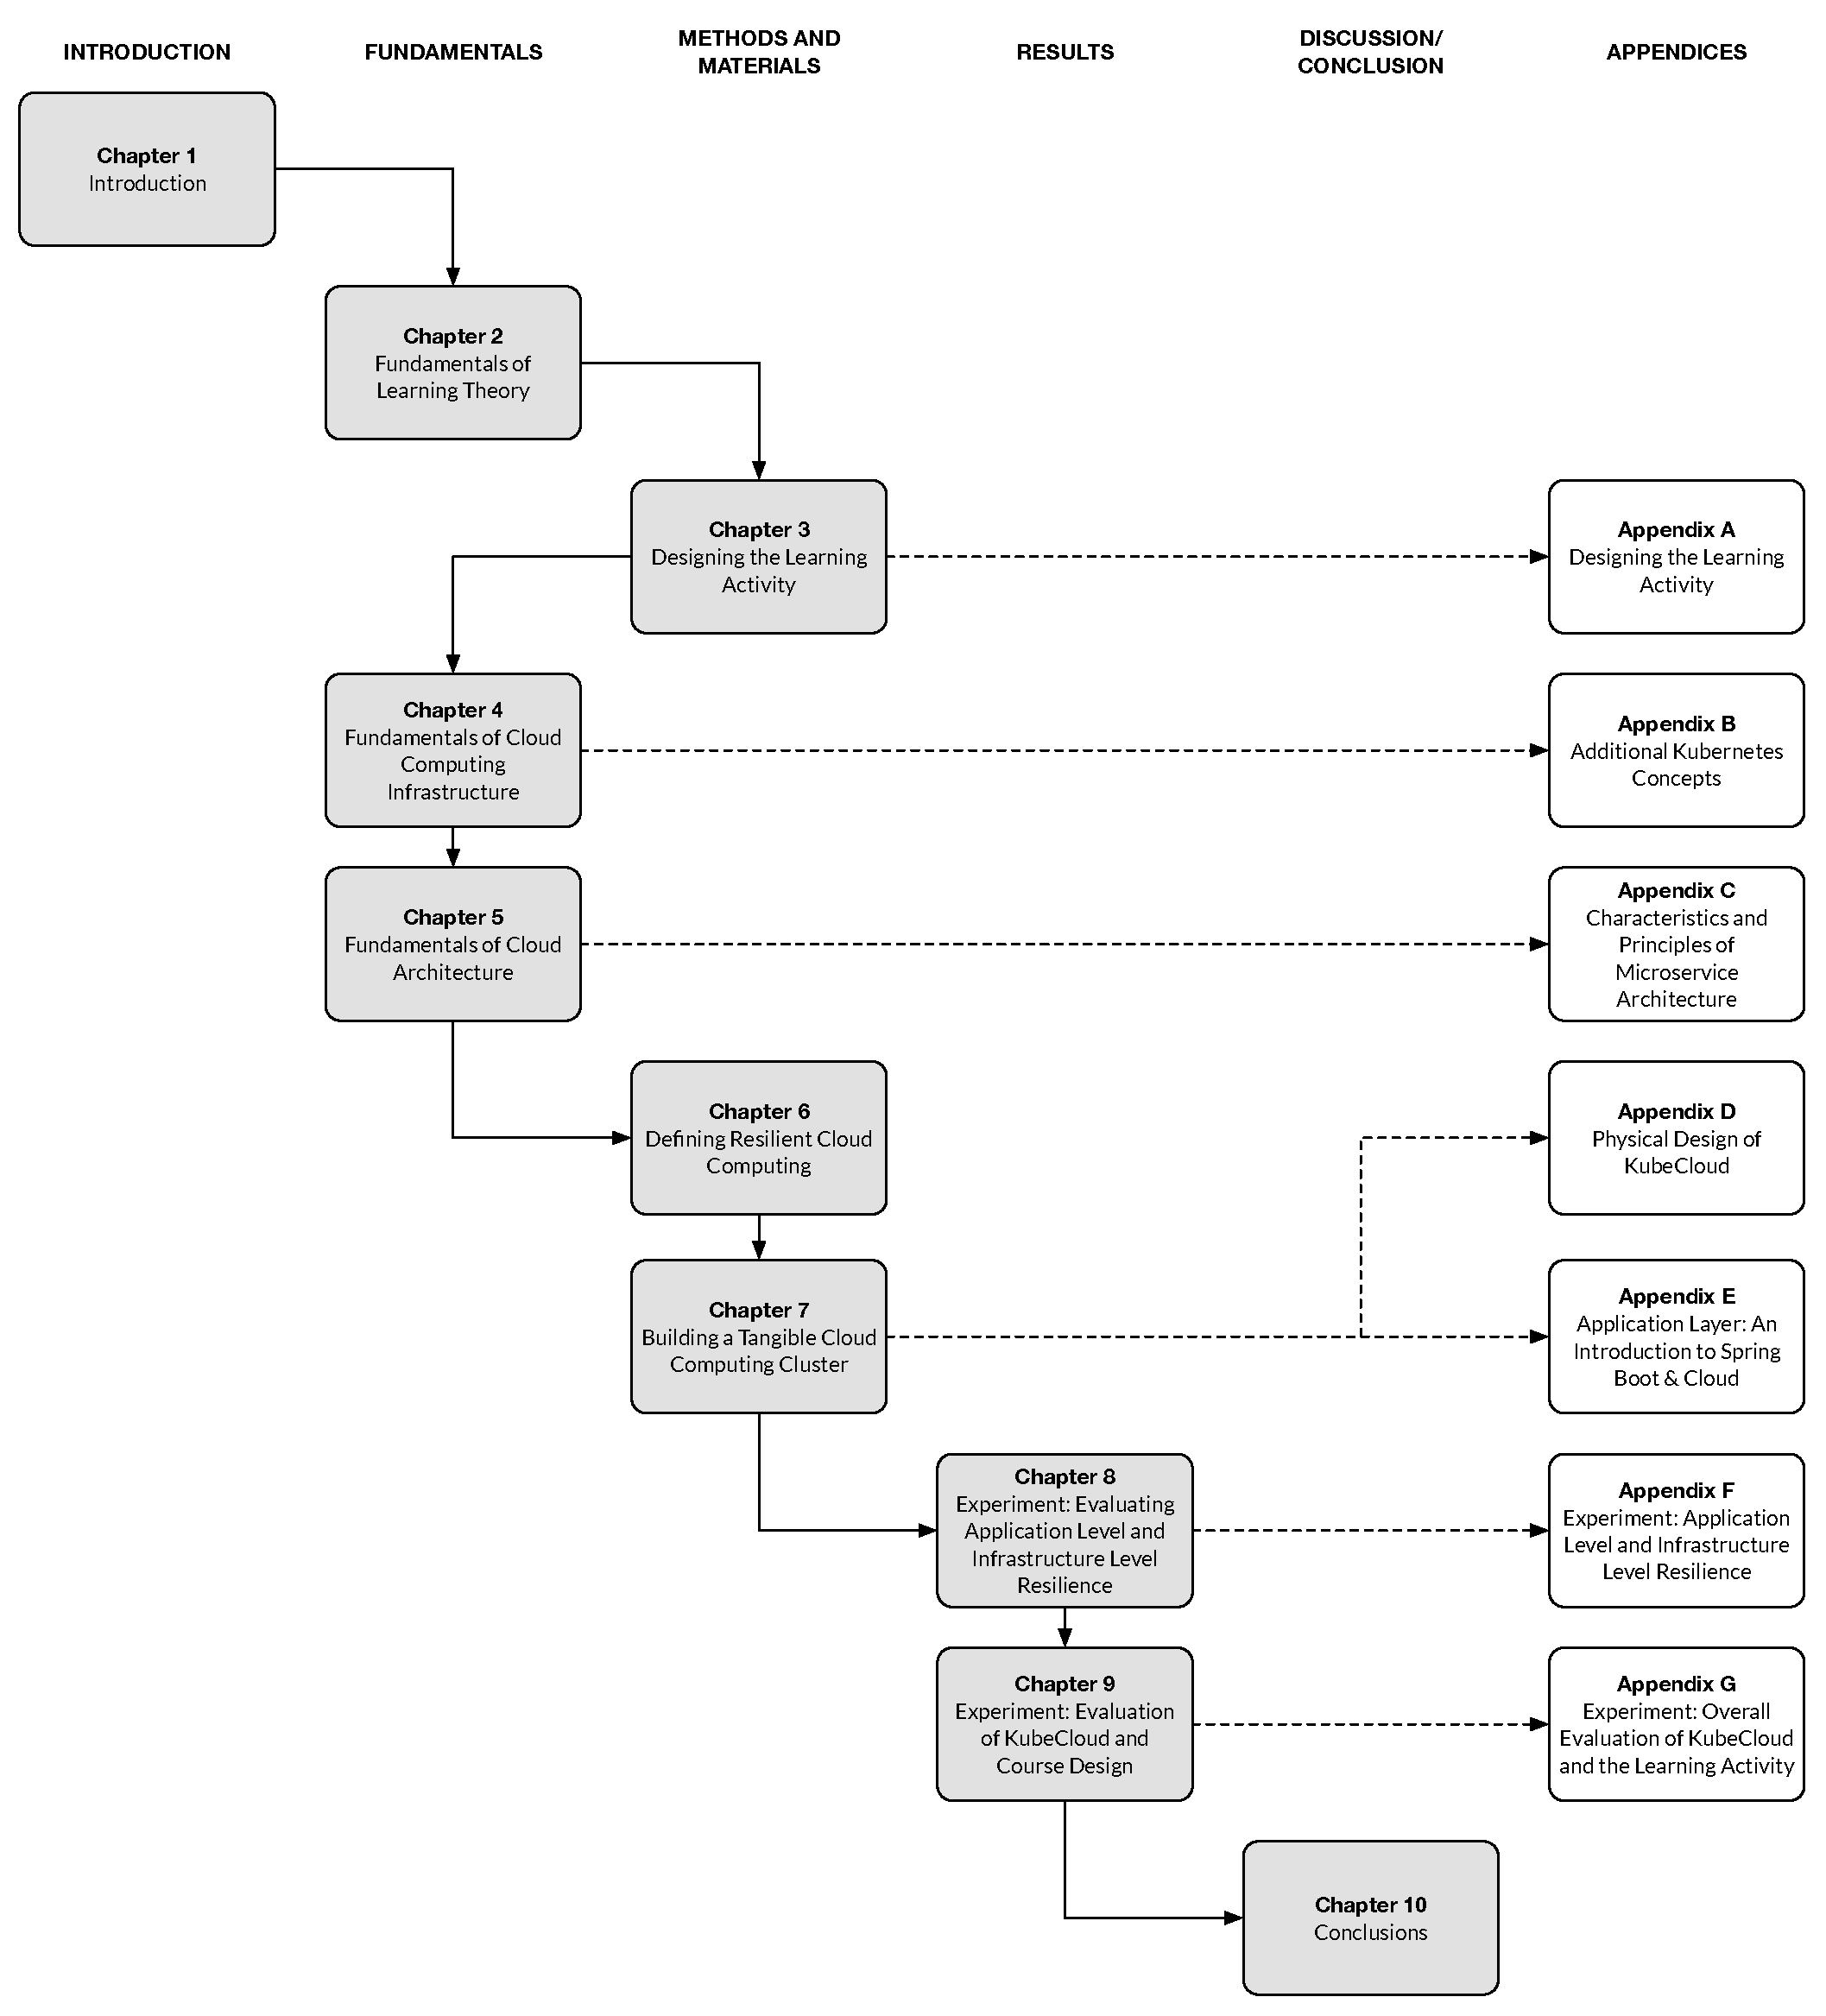
\includegraphics[width=13cm]{figures/thesis_structure}
\caption{Thesis Structure}
\label{fig:thesis_structure}
\end{figure}
